\section{Introduction}

Positive selection is a fundemental force in population genetics, and selective sweeps are responsible for many well-known examples of adaptation such as
changes in melanin production in humans \citep{williamson2007localizing},
insecticide resistance in \textit{Drosophila} \citep{schlenke2004strong}, and a major
architectural differences between teosinte and maize \citep{clark2004pattern}.
The foundational model of a selective sweep
describes how a novel, positively selected variant 
increases in frequency and eventually fixes \citep{fisher1930, kojima1962survival}. 
During this process, neutral variants linked to the sweeping variant also increase in frequency,
ultimately reducing variation around the site of the sweeping allele (i.e. genetic hitchhiking; \cite{smith_hitch-hiking_1974, kojima1967survival}).
This observation has been the basis of numerous tests for identifying positive selection in genomic data,
including those based on summary statistics \citep{tajima1989statistical, fay2000hitchhiking}, explicit likelihood models \citep{nielsen_genomic_2005, degiorgio2016sweepfinder2, chen2010population, degiorgio2022spatially},
and more recently through the use of supervised machine learning \citep{schrider2016s, kern_diploshic_2018, sugden2018localization, xue2021discovery, arnab2023uncovering, lauterbur2023versatile}.
However, this foundational model of a selective sweep - and the methods based on it - assume populations are panmictic and without spatial heterogeniety.
While these assumptions simplify models of sweeps, they also overlook
potentially confounding variables, as well as those that could better inform analysis.

One such factor is that most natural populations
live in landscapes where their dispersal and interactions are geographically limited, 
leading to a near ubiquitous observation in population genetics - isolation by distance (IBD) - 
that individuals tend to be more closely related the closer they are in geographic space \citep{wright_isolation_1943}.
This effect of spatially limited dispersal can have profound impacts on how genetic variation
is shared among individuals in a population, both with respect to common summaries of variation 
such as heterozygosity and the site frequency spectrum, as well as downstream inferences based on 
that variation such as inferred effective population sizes and genomic association tests \citep[e.g.,][]{battey_space_2020}.
These effects have implications for the ways that evolutionary processes, such as selective sweeps, are identified in natural populations.

Prior investigation into selective sweeps in spatially structured populations has revealed that a beneficial allele will move across space and through the population
as a travelling wavefront, historically described in a one-dimensional population by \cite{fisher_wave_1937} and in two dimensions by \cite{KPP1937}.
In this model, dispersal distance determines the speed at which a sweep progresses,
with smaller dispersal distances slowing the allele's frequency trajectory relative to the panmictic expectation \citep{barton_genetic_2013}.
\cite{min_spatial_2022} demonstrated how structure across one-dimensional space 
impacts the population genetic signatures expected after a selective sweep, 
most notably causing an excess of variants at moderate frequency that were able to
recombine onto the sweeping haplotype due to the slower nature of the sweep.
Further, \cite{chotai_signatures_2024} recently explored the signatures of sweeps in 
populations structured across continuous two-dimensional space.
This study corroborated results from one-dimensional explorations of sweeps in showing how sweeping alleles move more slowly in spatially structured populations
and demonstrated that spatial structure ``softens" the genetic signals expected from selective sweeps, causing them to appear more like soft sweeps \citep[\textit{c.f.},][]{hermisson2005soft}.
While our understanding of how spatial population structure changes expectations for the genetic signatures left by selective sweeps has increased, 
particularly in how it may reduce our capacity to detect them in genomic data, 
it remains unexplored whether this structure can be leveraged to inform genetic analysis of positive selection.

Spatial patterns of genetic variation
can reveal information about evolutionary process, rather than simply confound.
For example, \cite{battey_predicting_2020} showed how machine learning approaches
to geo-referenced data allow for geolocation of genotypes across continuous landscapes,
and that the residuals from such predictions can be used to infer historical processes \citep{battey_predicting_2020, rehmann2024evaluating}.
Further, spatial genetic data can be used to infer how organisms move across landscapes 
\citep{rousset1997genetic, ringbauer2017inferring, al2019estimating, marcus2021fast, smith2023dispersal, smith2023dispersenn2} 
as well as give information about local density of the population \citep{al2019estimating, smith2024estimation}.
While spatial data has been being utilized to inform genetic analysis of explicitly spatial processes, 
other fundamental phenomena, such as selective sweeps, are also impacted by spatial population structure.
Given that selective sweeps in spatially structured populations behave differently from those in panmictic populations, 
most notably in their speed and the impact of that on linked neutral variation,
this spatial dimension of how genetic variation is shared may contain information that reveals sweeping alleles.

Identifying selective sweeps is of particular importance in populations relevant to human health, 
such as the malaria-causing parasite \textit{Plasmodium} and its vectors.
The malaria vector \textit{Anopheles} is under strong selective pressures from public health interventions \citep[e.g.,][]{bhatt2015effect},
and thus is frequently reported as having experienced or or is currently undergoing selective sweeps in part due to these efforts \citep{anopheles2017genetic, clarkson2021genetic, xue2021discovery}. 
Genomic surveillance in these populations is crucial, as variants under positive selection are notably often in genes related to insecticide resistance, \citep{hemingway2016averting, clarkson2021genetic}, 
and thus relevant to advances in vector control and prevention of disease transmission.
While that is so, the studies identifying these variants often rely on methods that may be confounded by spatial population dynamics, reducing their power to identify sweeping alleles.
By using spatial information to inform searches for selective sweeps, we may be able to identify more (or different) variants under positive selection.

In this study, we use forward-in-time simulation to model selective sweeps across a continuous landscape and leverage the joint distribution between an allele's spatial spread and its frequency to reveal a novel signal of positive selection. 
We demonstrate this spatial signal's potential to reveal alleles under positive selection both through SNP-centric and windowed approaches, 
then apply these methods to a spatially referenced dataset of \textit{Anopheles gambiae} genomes \citep{malariagenAg1000GSelection}. 
Our analysis recovers known instances of positive selection in \textit{An. gambiae}, identifying variants within known insecticide-resistant loci,
and identifies potentially novel sources of insecticide resistance as well as other potentially selected variants
associated with immune response, sensory perception, and development.
Through simulation and empirical analysis, we demonstrate the potential of spatial population structure to identify, rather than obscure, segregating variants under positive selection.

\section{Methods}

\subsection{Spatial simulation}\label{subsec:spatial-simulation-method}

To simulate selective sweeps in continuous space, 
we used a \texttt{SLiM v3}  \citep{haller_slim_2019} model as described in \cite{battey_space_2020}
and elaborated on in \cite{chevy_population_2024}.
We model selection by having a selected allele modify mortality of its carriers
rather than fecundity. 
Following \cite{chevy_population_2024}, 
we define $f(u)$ as the per-capita mean number of offspring and $\mu(u)$ as the probability of mortality per unit time at local population density $u$, meaning the population reaches an equilibrium density when $f(u)$ and $\mu(u)$ are equal.
A positively-selected allele has additive effects ($h = \frac{1}{2})$ such that an individual with $k$ copies of the allele has a reduced mortality $\mu_k(u) = 1-(1-\mu(u))(1+\frac{ks}{2})$.
The positively-selected allele initially grows in copy number at a rate $G(u) = (1-\mu(u))(1+f(u))(1+\frac{s}{2})-1$, and because individuals carrying the allele have reduced mortality $\mu_k(u)$, its spread ultimately causes population density to increase (similar to what was observed in \cite{chevy_population_2024}).

Individuals were simulated across a 25 $\times$ 25 unit square continuous landscape 
with an initial average population density of 5 individuals per unit square area.
Over the course of a simulation time step,
individuals mate with proximate individuals,
newly born individuals disperse from their focal parent, then living individuals on the landscape compete locally for resources and space.
Mating, dispersal, and competition distances were drawn from a Gaussian kernel with mean zero and SD $\sigma$, which was varied between $0.40$, $1.25$, and $4.0$ to achieve initial Wright neighborhood sizes between 10, 100, and 1000 
(though these values changed as the sweeping allele spread and population density increased).
%Population size was controlled by calculating individual fitness based on local density such that the probability of an individual dying at locally-scaled population density $u$ can be expressed as $\mu(u)$,
%and therefore was impacted by the presence of the sweeping allele.
%More precisely, the probability of mortality for an individual with $k$ copies of an allele with selection coefficient $s$ becomes 
%$\mu_{k}(u)=1-(1-\mu(u))(1+\frac{ks}{2})$,
%ultimately causing population density to increase as the allele spreads across the landscape.
%Additionally, this density increase scales with the strength of selection, as described in \cite{chevy_population_2024}.
%population density increased as the sweeping allele spread, and this density increase scaled with the strength of selection (as described in \cite{chevy_population_2024}).

Each individual had a diploid 10\textsuperscript{8} bp genome that recombined at
a rate of 10\textsuperscript{-8} per bp per generation. 
After an initial burn-in of 1000 time steps, 
a positively selected mutation with a selection coefficient chosen from  [$1\times10^{-4}, 0.001, 0.01, 0.1$] was added to the center of a chromosome from 
a newly born individual at the center of the landscape.
As the simulation progressed, the frequency of the sweeping allele was tracked,
alongside the landscape area occupied by individuals carrying the sweeping allele, 
calculated as the area of the convex hull containing all allele carriers \citep{barber_quickhull_1996}.
We ran 100 total simulations to fixation across each parameter combination; simulations where the allele did not fix were restarted from the time point just before the addition of the sweeping allele.

\subsection{Power analysis}\label{subsec:power-analysis}

To assess the power of this spatial signal to identify variants under positive selection,
we analyzed the spatial distribution of neutral variation across the genome over the course of our simulations.
From each previously described simulation, we saved tree sequences over the course of the sweep 
(at a rate of 1 tree per 1 time step for a selection coefficient of 0.1,
2 time steps for 0.01, 5 time steps for 0.001, and 10 time steps for $1\times10^{-4}$, respectively).
Tree sequences were saved at different rates for different selection coefficients in order to capture the full dynamics
of allele frequency while reducing computational time and memory load \citep{treeseq}.
%Increasing the sampling of tree sequences with selection coefficient was important to capture the full dynamics of allele frequency and area change during the simulated sweep.

After simulating, we used \texttt{msprime} version 1.3.1 \citep{baumdicker_efficient_2022} to recapitate the tree sequence, adding neutral mutations to the genome based on a population size equal to the population size at the tenth time step of the simulation (after which the population was spatially established), using a mutation rate of 10\textsuperscript{-8} per bp per generation.
We then measured the frequency and area (through the same methods described in Methods \nameref{subsec:spatial-simulation-method}) of each variant across the genome, taking note of the sweeping allele.
We used the joint distribution between allele frequency and occupied area of all variants across the genome to identify spatial-frequency (SF) outliers by
binning every 1,000 variants (grouped by frequency), then classifying the lower $Nth$ percentile in regards to area of these groups as spatial-frequency (SF) outliers 
(Figure \ref{fig:poweranalysis} A).
To assess our power to identify the sweeping allele based on the joint distribution between frequency and area, 
we tested for the presence of the sweeping allele among these SF outliers while varying the percentile cutoff between $0.5$ and $0.01$. 

Additionally, we analyzed the ratio of
SF outliers to non-outliers in 100kb windows along the genome (Figure \ref{fig:poweranalysis} B). 
To prevent our analysis from being thrown off by windows without many variants,
we used as our statistic a $Z$-score defined as
$$Z = \frac{\frac{O}{S} - Q}{\sqrt{Q \times \frac{(1 - Q)}{S}}}$$
where $O$ is the number of SF variants in a window, $S$ is the total number of variants, and $Q$ is the genome-wide proportion of SF outliers to all variants.
Genomic windows that had SF outlier:non-outlier ratios above the Nth percentile of genome-wide ratios
were identified as windowed spatial-frequency (WSF) outliers while again varying the percentile cutoff between $0.5$ and $0.01$, and 
we again tested for whether the sweeping allele was identified as being within a WSF outlier window.

\subsection{\textit{Anopheles gambiae} analysis}

\subsubsection{Data processing}

We applied our method to whole genome sequencing of \textit{Anopheles gambiae} available through the \ag project \citep{consortium_genome_2020}. Genotype data and metadata were downloaded from the \ag phase 3 (Ag3.0) data release (accessed April 2024; https://malariagen.github.io/vector-data/ag3/ag3.0.html). VCFs relating to 28 sampling sets were merged using \texttt{bcftools} v1.20 \citep{bcftools} and the command ‘merge’ with default options. Metadata were filtered to identify \textit{An. gambiae} individuals as defined in the metadata header: 'aim\_species' and 'taxon'. The merged VCF was filtered to retain only those \textit{An. gambiae} individuals, resulting in 1470 individuals for downstream analyses. Monomorphic sites were removed using \texttt{bcftools} v1.20 and command ‘filter’ with options -e 'AC==0 \textbar\textbar AC==AN'. Finally, the VCF was filtered to retain high quality sites and accessible regions of the genome using the site filters available through Ag3.0. The final VCF contained 83,924,645 polymorphic sites, where 28\% were classified as multiallelic (\textgreater 1 alt allele). 

The allelic state was polarized using the program \texttt{est-sfs} v2.03 \citep{keightley2018inferring} with \textit{An. coluzzii}, \textit{An. arabiensis}, \textit{An. melas}, and \textit{An. merus} as outgroup species. \textit{An. coluzzii} and \textit{An. arabiensis} are part of the Ag3.0 data release, and their VCFs were downloaded and processed in the same methods as outlined above. These VCFs were also filtered to retain only individuals with an unambiguous species identification. This left a total of 507 individuals of An. coluzzii and 368 individuals of \textit{An. arabiensis}. The two other outgroup species, \textit{An. melas} and \textit{An. merus}, were downloaded from the available data sets of \cite{fontaine2015extensive}. An input file for \texttt{est-sfs} was constructed using the custom script \texttt{estsfs\_format.py} to partition the VCF into files with 100,000 sites for fast parallelization. The program est-sfs was then run with default parameters and the results integrated back into the \textit{An. gambiae} VCF by adding an Ancestral Allele (AA) state to the INFO column of the VCF. The ancestral allele was determined to be the reference allele if the probability given by est-sfs was \textgreater 0.90 and then the alternate allele if 1-probability was \textgreater 0.90. Parsimony was used to polarize all other sites that could not be confidently polarized from the \texttt{est-sfs} results.
Impacts of derived alleles were then annotated onto the VCF using \texttt{SNPEff} v5 and the AgamP4 reference genome (Assembly GCA\_000005575.1) \citep{cingolani2012program}.

To reduce impacts of larger-scale population structure, we focused our analysis on 687 \textit{An. gambiae} samples from West Africa grouped using \texttt{ADMIXTURE}. Ancestral clusters were estimated using \texttt{ADMIXTURE} \citep{alexander2011enhancements}. A VCF of the genomic regions 3R:1-37,000,000 and 3L:15,000,000-41,000,000 (as noted in \cite{anopheles2017genetic}) were filtered to retain SNPs with a minor allele frequency \textgreater 5\% and then thinned to retain only 1 site every 5,000bp. Thinning was done to reduce the influence of site dependency via linkage. The VCF was converted to bed format using \texttt{PLINK} v1.9 \citep{purcell2007plink}. \texttt{ADMIXTURE} was run for a K from 1 to 5 (number of ancestral populations) with 5-fold cross-validation. Each \texttt{ADMIXTURE} analysis was repeated 30 times with different seeds. Final groups were visualized using \texttt{CLUMPAK} \citep{kopelman2015clumpak} and individuals were then assigned to one of the three clusters, the optimal K being 3 using an admixture proportion cutoff of 0.88.

A recombination map was estimated using \texttt{ReLERNN} v1.0.0 \citep{adrion2020predicting} and mosquito sequences collected from the Central African Republic (CAR) (see Ag3.0 data release). The CAR population was used because sampling among the other \textit{An. gambiae} populations was variable in both time and space. In contrast, CAR had 55 female mosquitoes collected during the same year (1994) and location (Bangui).
\texttt{ReLERNN} was run on the phased and filtered VCF containing mosquitoes from CAR and a mask file (MASK) denoting the non-accessible regions of the genome. A custom demographic history (DEMO) trajectory for CAR mosquito population was inferred using \texttt{StairwayPlot2} \citep{liu2020stairway}. The classifier was trained using a window size of 26,000bp with default options and setting required parameters: --assumedMu $3.0e-9$ --upperRhoThetaRatio 30 --phased --mask $MASK -n $DEMO. The resulting recombination maps were translated to cM/Mb and HapMap3 format using a custom script \texttt{rho2cMMb.py}. 

\subsubsection{Spatial genome scan} \label{ag-genome-scan}

We applied our analysis to 687 \textit{An. gambiae} samples from West Africa grouped using \texttt{ADMIXTURE}.
We recorded the frequency of each variant globally within the sample population
alongside the area of the landscape occupied by its carriers.
The area of the landscape occupied by allele carriers was determined by fitting a convex hull over the sampling locations
of individuals carrying the allele through the same methods described in Methods section \nameref{subsec:spatial-simulation-method}, then calculating the area (in square kilometers) of the polygon determined by this hull using \texttt{pyproj.Geod}.
Alleles that were not present in at least three unique locations were discarded from our analysis as we were unable to determine the area occupied by these variants.

From the joint distribution of allele frequency and area, we identified SF outliers as those below 
a spline fit (using the R package \texttt{npreg}) through the lower tenth area percentile of every 1000 SNPs binned by frequency after removing SNPs within the three major inversions (2La, 2Rb, 2Rc).
To characterize the ``distance'' of an individual SNP from this cutoff, we used
a modified $z$ transformation of each SNP's area compared to the distribution of areas within
the defined 1000-SNP frequency bin, centering the areas according to the median of the distribution and then scaling by the median absolute deviation of the distribution. Such $z$ scores give us a sense, although imperfect, 
of the strength of the outlier relationship.
We then used a 100kb windowed analysis to identify WSF outliers beyond the 90th percentile of genomic $z$ scores of SF outlier:non-outlier SNPs. This same approach was applied separately to SNPs within each the three major inversions (Figure \ref{fig:inversionjdist}).
To prevent regions with low variation from inflating genome-wide $z$ score values,
we masked windows with a recombination rate below 1.5 cM/Mb before placing the 90th percentile cutoff to identify WSF outlier windows.

To assess potential phenotypic impacts of SF and WSF outliers,
we searched for enrichment of SNP annotations obtained using SNPEff \citep{cingolani2012program} using a $\chi^{2}$ test. 
Next, we identified genes containing SF and WSF outliers using VectorBase \citep{giraldo2015vectorbase}, then used this list of genes to search for enrichment of functional annotations using either \texttt{PANTHER} (for SF outliers) or \texttt{DAVID} (for WSF and NS outliers) \citep{panther, Mi2019-od, dennis2003david}.
Finally, for nonsynonymous WSF outliers, we obtained \texttt{.pdb} files of predicted protein structure for their associated genes using \texttt{AlphaFold3}, 
then used \texttt{ThermoMPNN} to assess how the associated amino acid substitution impacted protein stability \citep{jumper2021highly, dieckhaus2024transfer}.
For \textit{CYP4H27}, we used the pairwise structure alignment tool available via \url{www.rcsb.org/alignment} with method \texttt{TM-align} to compare the ancestral and derived versions of the protein \citep{pdb-align}.


\section{Results}

\subsection{A novel spatial signal of selection}

How does a beneficial allele move across space? 
An allele under positive selection that arises at a point along the landscape
(position 50 in Figure \ref{fig:alleleviz}) will increase in frequency where it arises while simultaneously 
spreading in all directions in the form of a traveling wave \citep{fisher_wave_1937, KPP1937}.
While the beneficial allele is globally increasing in frequency, 
the portion of the landscape occupied by carriers of said allele 
is constrained by the wavelike dynamics of its spread. 
%the standing wave dynamic constrains the portion of the landscape that carriers of the selected allele occupy.
In contrast, a neutral allele that arises and is not lost will diffuse in both directions,
but generally remain at low or intermediate frequencies across the landscape, as its frequency dynamics are determined by drift (Figure \ref{fig:alleleviz}).
Because positive selection causes a beneficial allele to increase in frequency faster than it can spread through space, these alleles should occupy less space on the landscape than neutral variants at similar global frequencies.
We set out to observe this phenomenon in continuous space using forward-in-time, individual-based simulation.

\begin{figure}[htp]
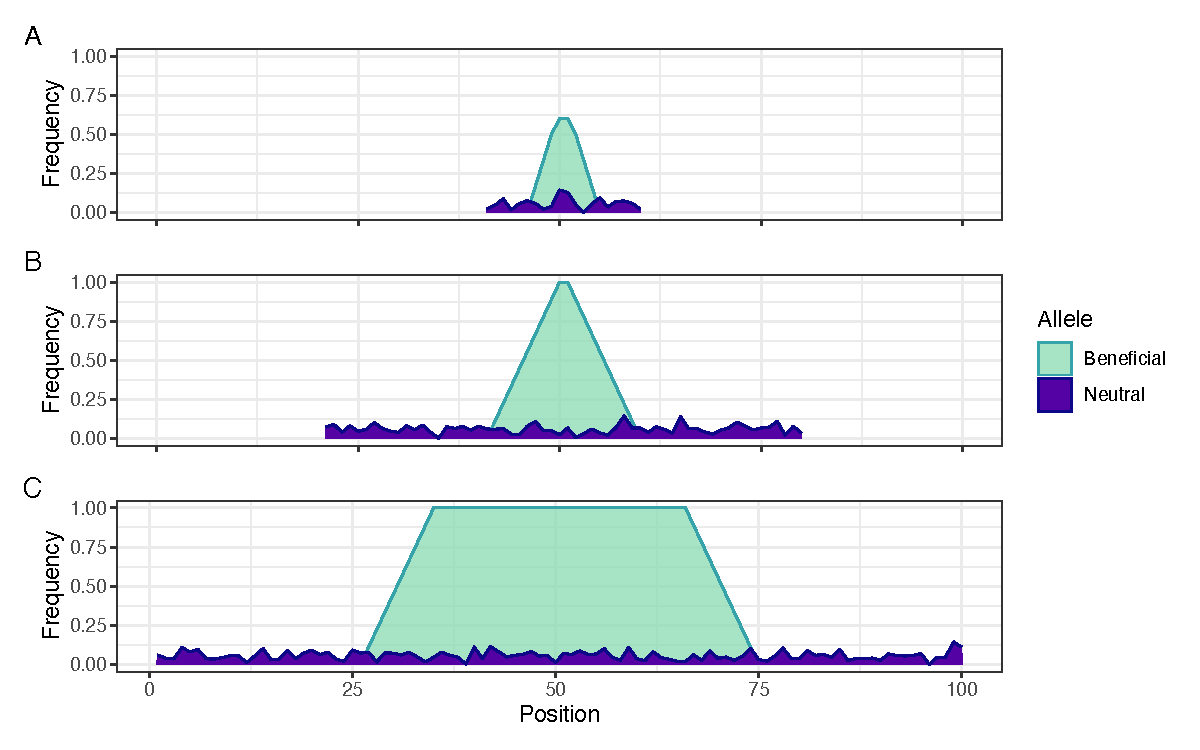
\includegraphics[width=\linewidth]{{figures/allele_conceptviz.pdf}}
\centering
\caption{A conceptual model of how positive selection impacts an allele's spread across a one-dimensional landscape.
Panels A, B, and C show a time series of a beneficial allele (in green) and a neutral allele (in blue) arising at position 50 and spreading through space.
The frequency of each allele at a given spatial position is indicated along the y axis.
}
\label{fig:alleleviz}
\end{figure}

To simulate selective sweeps in continuous space,
we used a non-Wright-Fisher framework similar to that described in \cite{chevy_population_2024}, 
where individuals disperse from their parent across the landscape, compete locally for resources, and reproduce with a spatially proximate mate.
Dispersal and interactions are governed by a Gaussian kernel with size $\sigma$, which represents the 
average per-generation movement rate, competition distance, and mate search radius (Methods \nameref{subsec:spatial-simulation-method}).
%where individuals disperse across the landscape according to a Gaussian dispersal kernel parameterized by
%the average per-generation movement rate $\sigma$. Reproduction is local, with a Gaussian mate choice kernel also set
%to $\sigma$, and population size is regulated by local density dependence.
On to this continuous space simulation we introduce a positively selected allele -- one that reduces individual mortality -- to the middle of the simulated genome of an individual at the center of the landscape, 
then track the progress of the focal mutation until eventual fixation or loss (Figure \ref{fig:sweepsim}A).
Additionally, we compare results of our simulations to simple theoretical deterministic expectations
of the spread of a beneficial allele according to traveling wave dynamics (Supplemental section \nameref{sec:S1}; \cite{fisher_wave_1937, KPP1937}).
In our simulations, we tracked the frequency of the allele as well as the area of the landscape occupied by the allele's carriers, where area was defined by a convex hull formed
at the vertices of allele carriers (see Methods).

In Figure \ref{fig:sweepsim}B we show the allele frequency and area trajectories resulting from our spatial simulations.
In accordance with the conceptual model shown in Figure \ref{fig:alleleviz}, alleles under strong positive selection occupy less space on the landscape in comparison to neutral or weakly selected alleles at similar frequencies.
There is a strong relationship between the strength of selection, the frequency of a beneficial allele, and its area:
as the strength of selection increases, beneficial alleles cover \textit{less} of the landscape
conditional on frequency.
This effect is most pronounced at smaller dispersal rates, 
where the allele's spread is inherently more limited by spatial population structure,
but persists even when per-generation dispersal is high. 
Selection's effect on this joint distribution - reducing relative area - 
is initially counterintuitive as one might expect a sweeping allele to spread more quickly
across a landscape than a neutral variant. This is true with respect to time, 
however conditional on its frequency, a neutral variant will diffuse across the landscape without a substantial increase in frequency.
Under positive selection, an allele will both spread across the landscape and increase in frequency,
reducing the expected area associated conditional on frequency and creating a visible signal in the joint distribution (Figure \ref{fig:sweepsim}B). We note that deterministic models of Fisherian wave dynamics recapitulate these dynamics as well (Figure \ref{fig:fisher}), thus drift is not responsible for the general effect.

\begin{figure}[htp]
\includegraphics[width=\linewidth]{{figures/sweepsimjointdistribution.pdf}}
\centering
\caption{Selective sweeps in continuous space. 
(A) Example of simulated allele with selection coefficient 0.1 
sweeping through a population with a dispersal distance ($\sigma$) of $0.40$.
Individuals carrying the sweeping allele are colored in green.
(B) Joint frequency-area trajectories of sweeping alleles at dispersal distances
$0.40$, $1.25$, and $4.0$. 
Line color represents the strength of selection; 
allele area is measured as the area of the polygon encompassing allele carriers.}
\label{fig:sweepsim}
\end{figure}

\subsection{Power to detect selection using space}

We next asked whether we could use this spatial signal to identify alleles under positive selection.
Given that positive selection has a striking impact on allele area conditioned on frequency,
we decided to use an empirical outlier approach on this joint distribution to localize candidate selected alleles. 
Simply put, the idea is to 
%define a cutoff in the genome-wide joint distribution of allele frequency and area in order to 
identify alleles that occupy less area than expected given their frequency (spatial-frequency or SF outliers).
An example of this joint distribution along with a heuristic cutoff to identify SF outliers is shown in Figure~\ref{fig:poweranalysis}A.
While this distribution is defined based on individual SNPs, 
sweeping alleles also bring along their linked genetic background, 
and there may be additional power in aggregating SF outlier signal across windows.
%While we are defining this distribution based on individual SNPs, because
%sweeping alleles bring along their linked genetic background, there may be additional power in taking a genomic window 
%approach as well.
To do so, we first identify genome-level SF outliers (as in Fig.~\ref{fig:poweranalysis}A) in a genomic window, then
define a $z$-score from
the proportion of variants found within a given window that are SF outliers (see \nameref{subsec:power-analysis} section). 
The goal is to identify particular windows
which harbor an excess of spatial-frequency outliers (WSF outliers, see \nameref{subsec:power-analysis}; 
Figure~\ref{fig:poweranalysis}B).

We characterized power of the spatial-frequency (SF) outlier and windowed (WSF) outlier methods using 
forward-in-time spatial simulations for differing combinations of selection coefficients
and dispersal rates ($\sigma$)
while varying the stringency of the empirical cutoff used to define outliers. 
Unsurprisingly, we found that our method is best powered to detect the sweeping allele
when the strength of selection is strong and dispersal is limited
(Figs.~\ref{fig:poweranalysis}C and \ref{fig:poweranalysis}D).
Using an empirical cutoff at the $10^{th}$ percentile leads to 
a reasonable balance of power and false positive rate given the parameterization of our
simulations (Figs.~\ref{fig:poweranalysis}C and \ref{fig:poweranalysis}D), here observed
as an inflection point in our power curves. We thus chose this cutoff for later empirical analysis. 

Across all dispersal distances and selection coefficients, the probability of detecting the sweeping allele changes as a function of its frequency and increases sharply as the allele reaches fixation (Figure \ref{fig:poweranalysisoutlierprop}).
Because there are fewer high-frequency SNPs overall and the landscape area they occupy is inherently high, we become more likely to identify the sweeping allele as an outlier in the joint distribution.
Variation that is linked to this sweeping allele is also likely to take up less area relative to its frequency, contributing to power to detect the genomic window containing the sweeping allele.

While our method demonstrates potential to detect in-progress sweeps, its empirical approach also results in a number of false positives that we control based on the defined outlier cutoff.
For example, in our simulations with a single SNP under selection,
identifying the lower tenth percentile of the joint area-frequency distribution as SF outliers and the upper tenth percentile of windowed SF outlier ratios as WSF outliers resulted in roughly $20,000$ SNPs (10\% of genomic variation) being identified as SF outliers and roughly $3400$ SNPs (less than 2\% of genomic variation) being identified as WSF outliers.
In empirical applications, genomic/biological annotations can help deal with sorting through these SNPs.

\begin{figure}[htp]
\includegraphics[width=\linewidth]{{figures/poweranalysisres.pdf}}
\centering
\caption{Power to detect selective sweeps using continuous space.
(A) Example genome-wide joint distribution between frequency and area of all variants 195 time steps after the introduction of an allele with a selection coefficient of $s=0.1$ in a population with a mean per-generation dispersal distance of $0.40$.
The black line represents the tenth percentile cutoff for SF outliers; the sweeping allele is highlighted in green.
(B) Example genome-wide windowed analysis of the ratio of SF outliers to non-outliers at the same time point in the same simulation.
The dotted line represents the tenth percentile cutoff for WSF outliers; the green triangle highlights the locus of the sweeping allele.
(C) Probability of detecting the sweeping allele as a SF outlier as the strictness of the outlier cutoff increases along the x axis. Panels represent $\sigma$ values $0.40$, $1.25$, and $4.0$; line color represents the strength of selection. The dashed gray line represents the proportion of the genome identified as SF outliers.
(D) Probability of detecting the sweeping allele as a WSF outlier in the same simulations; the dashed gray line represents the proportion of the genome identified as WSF outliers.
}
\label{fig:poweranalysis}
\end{figure}

\subsection{Spatial signal identifies sweeping alleles in \textit{Anopheles gambiae}}

After demonstrating the potential of this spatial signal to identify positively selected variants,
we next applied our approach to 
$687$ West African \textit{Anopheles gambiae} samples from the \ag project 
(spatial sampling shown in Figure~\ref{fig:agjoint} inset; data described in \cite{consortium_genome_2020}). 
Because this species is under strong selective pressures from human interventions, this is a useful system for testing our method with potential consequences for vector control efforts.
For each SNP in the genome, we recorded its global frequency along with the locations (in latitude and longitude) of individuals carrying that SNP.
After discarding SNPs that were found in fewer than three unique locations (706,991 alleles or approximately 71.2\% of genomic variation, leaving 297,305 SNPs used in our analysis),
we estimated the area on the landscape that each SNP occupies as the convex hull encompassing all individuals carring the allele.
Using the resulting distribution of SNP frequency and area, we used an empirical 10\% 
area cutoff, conditioned on frequency, to identify SF outlier SNPs (Figure \ref{fig:agjoint}).
%and characterized the potential functional impacts of this set of outlier loci
%on \textit{An. gambiae} phenotypes.

As above, because positive selection reduces the area an allele occupies conditional on its frequency,
we focused on SNPs in the joint distribution that match this pattern (Table S1).
As linkage betweeen SNPs might lead to genetic hitchiking between neutral and 
non-neutral SNPs, we further refined our analysis using a genomic scan to identify 100 kb windows of the genome that contain an excess of SF outliers after masking low-recombination regions, labeling SF outliers within these regions as windowed SF outliers (WSF outliers, Figure~\ref{fig:agwindows}).
To reduce the impact of other non-neutral processes on our analysis, we identified outliers separately for the major inversions (2La, 2Rb, 2Rc) and the rest of the genome, respectively, then SF and WSF outliers were pooled for downstream analyses. 
In total, we identified 36,500 SNPs as SF outliers 
%(approximately 3.7\% of genomic variants) 
and 3,875 SNPs as WSF outliers. %(approximately 0.4\% of genomic variants).
It's worth noting that our WSF outlier statistic agrees to some degree with previous searches for 
selective sweeps done in this system, and we find 
weak but significant correlations with windowed iHS statistics ($p = 4.658 \times 10^{-8}$; \cite{anopheles2017genetic}) and 
windows identified using partialSHI/C ($p < 2.2 \times 10^{-16}$; \cite{xue2021discovery}), providing independent evidence that we are 
indeed picking up signals of positive selection.


To assess what biological signals were being identified through our spatial approach,
we first investigated the SF outliers' annotations and associated genes.
SF outliers were significantly enriched for coding SNPs (5.86\% of SF outliers were located in coding regions compared to 5.31\% of all SNPs retained in our analysis), with significant enrichments for both synonymous ($p = 7.196 \times 10^{-7}$, $\chi^{2}$ test) and nonsynonymous variants($p = 0.046$, $\chi^{2}$ test) (Figure \ref{fig:agjoint}).
Furthermore, SF outlier SNPs that are significant outliers in the joint genome-wide distribution of frequency and area fall within a number of loci associated with insecticide resistance, including 
an intronic variant within the \textit{VGSC} locus (2L:2395567, $z = {-6.66}$; \cite{Martinez-Torres1998-pn}), 
31 intronic variants and 6 synonymous variants within the \textit{Cyp6p} locus (2R:28480576-28505816, $z$ scores range from ${-0.82}$ to ${-7.71}$; \cite{Muller2008-fo}), and
29 intronic variants within the \textit{Rdl} locus (2L:25363652 - 25434556, $z$ scores range from ${-0.66}$ to ${-13.21\times10^{10}}$; \cite{Du2005-iv}).
Beyond these loci, the genes containing SF outliers (both coding and noncoding) were significantly enriched after Bonferroni correction for a number of GO biological processes important for sensory processing, including action potential (2.84 times enrichment, $p = 1.64 \times 10^{-02}$), 
neuron recognition (2.63 times enrichment, $p = 1.92 \times 10^{-2}$), 
and axon guidance (2.38 times enrichment, $p = 1.21 \times 10^{-13}$) (Table S2).
Sensory perception and processing is often implicated in mechanisms of insecticide resistance in \textit{Anopheles} species, and these genes are likely under further selective pressures from other environmental factors and vector control measures.

\begin{figure}[htp]
\includegraphics[width=\linewidth]{{figures/anopheles_jointdistribution.pdf}}
\centering
\caption{
Joint distribution between frequency and area of all variants within the \textit{Anopheles gambiae} genome.
Each point represents a genomic variant; 
the point's color indicates its annotation. 
Outlier variants highlighted in vignettes are colored and outlined.
Black lines represent SF outlier cutoffs for each of the major inversions and the non-inverted portion of the genome, respectively.\linebreak{}
INSET: Sampling locations of \textit{An. gambiae} samples. The size of the points represents the number of samples at each location.
}
\label{fig:agjoint}
\end{figure}

We next turned to our windowed WSF outliers (Figure \ref{fig:agwindows}).
We again tested for enrichment of SNP annotations within these WSF outliers and found a significant enrichment of upstream ($<5$kb from the transcription start site) gene variants ($p = 8.004 \times 10^{-6}$, $\chi^{2}$ test) and intronic variants ($p = 1.015 \times 10^{-6}$, $\chi^{2}$ test), which may indicate that a substantial
portion of variants under positive selection are regulatory in this system.
Further, ten WSF outliers fall within a well-known locus of insecticide resistance, Ace1 (2R:3484107-3495790, $z$ scores range from $-1.03$ to $-2.67$).
Genes containing WSF outliers were also significantly enriched for drug metabolism function (Enrichment score = 2.41, $p = 0.0062$) and enriched, though not significantly, for other relevant functions and annotations, including
CRAL-TRIO domain-containing proteins, which are associated with eyesight (Enrichment score = 1.64, $p = 0.47$; \cite{smith_molecular_2015}) and
G protein-coupled receptors (Enrichment score = 1.78, $p = 0.96$, Bonferroni correction) (Table S3).

Finally, we searched for nonsynonymous outlier SNPs that could potentially be associated with functional changes.
Investigating the functional consequences of nonsynonymous outlier SNPs,
we found 37 WSF outliers and 237 SF outliers that impact protein stability (274 in total out of the 526 nonsynonymous outliers identified; Table S4).
Among these are 44 variants within genes potentially associated with insecticide resistance
as defined by the Ag1000g Selection Atlas,
including methylenetetrahydrofolate reductase (AGAP007479:Y174D, $z = -0.62$), 
heme peroxidase 7 (AGAP004036:E564D, $z=-0.86$), and cytochrome P450 enzymes
CYP6N2 (AGAP008206:K392N, $z=-0.76$), CYP4D15 (AGAP002418:L80M, $z=-0.88$),
and CYP4H27 (AGAP008552, highlighted below) \citep{malariagenAg1000GSelection}.
The largest stability changes were observed within genes coding for metabolic proteins,
which may be indicative of selective pressures exerted by insecticides, which target metabolic processes.
High-magnitude stability changes are also observed within genes involved in sensory function,
which may be due to changes in behavior associated with insecticide resistance \citep{Thomsen2016-hd}, 
and genes involved in the regulation of gene expression.
Changes in gene expression are often the mechanism behind insecticide resistance in \textit{Anopheles}
and other mosquitoes, and alterations in regulatory proteins may contribute to resistant phenotypes \citep{Muller2008-fo}.

\begin{figure}[htp]
\includegraphics[width=\linewidth]{{figures/aggenomicwindows_annotated.pdf}}
\centering
\caption{Genome-wide windowed analysis of the ratio of SF outliers to non-outliers. 
Flat horizontal lines represent WSF cutoffs for each of the major inversions and the non-inverted portion of the genome, respectively.
Known loci associated with insecticide resistance and outlier variants highlighted in vignettes are labeled.
}
\label{fig:agwindows}
\end{figure}


While there are a number of individual loci that we could highlight, in what follows we provide 
three particularly interesting vignettes of loci that represent strong spatial-frequency outliers in our scan and
may be of functional consequence (see Figure~\ref{fig:agmissense}).

\subsubsection{Cytochrome P450 \textit{CYP4H27}}

Cytochromes P450 are frequently implicated in the evolution of insecticide resistance across multiple taxa.
In \textit{Anopheline} mosquitoes, positive selection linked to Cyp450-associated resistance is most often associated with increased protein expression level due to copy number or transcriptional changes, rather than changes in protein function \citep{Muller2008-fo}.
However, using our SF outlier approach, we identify three nonsynonymous variants within one cytochrome P450 \textit{CYP4H27} (Gene ID AGAP008552) that impact the folding stability and binding site conformation of this protein (Figure~\ref{fig:agmissense}A). 
The first variant of interest, 3R:12573245T$>$C, is found only in five sampling locations, but is at a global frequency of almost 40\%, and thus represents a highly significant outlier from the genome-wide joint distribution, the strength of which we can characterize with a $z$-score ($z = -12.61$).
This mutation results in a shift from tyrosine to histidine at amino acid position 274 (Y274H) within the G helix of the CYP4H27 protein. 
The substitution shifts the orientation of the S326 residue on the N-terminal end of the I helix within the protein's active site, allowing it to join a helix-stabilizing hydrogen bond between the residues of E327 and S324 and the carboxyl group of E27 and
reducing the volume of the ligand binding pocket from $630.271 \text{ \r{A}}^{3}$ to $595.784 \text{ \r{A}}^{3}$ as modeled by AlphaFold2 predictions \citep{castpfold, alphafold}.
Given that positively selected Cyp450 variants tend to be associated with increased protein expression that aids with insecticide detoxification, this modification to the structure of the CYP4H27 active site may have implications for its enzymatic activity, however further investigation is required to confirm this.

The other two variants of interest, 3R:12573798A$>$C and 3R:12573814T$>$A, are at 54\% and 49\% frequency ($z = -2.62$ and $z=-10.36$), respectively, 
and both result in charged amino acid changes between the L and M helices:
3R:12573798A$>$C causes a negatively charged serine at position 458 to change to a positively charged arginine (S458R),
and 3R:12573814T$>$A causes a nonpolar valine at position 463 to change to a negatively charged aspartic acid (V463D).
Among the individuals analyzed, we identified three mosquitoes with both the Y274H and S458R mutations segregating on the same haplotype
and three mosquitoes with both Y274H and V463D segregating together, though we were unable to definitively find one haplotype with all three variants.
AlphaFold predictions of the S458R and V463D carrying structures suggest these amino acid substitutions occur at the entrance of the ligand binding pocket, shifting its conformation, and that these changes are amplified when in combination with the Y274H mutation.
Though the phenotypic effects of these three Cyp450 variants needs to be further investigated \textit{in vivo}, their strong signals of positive selection may indicate another Cyp450-mediated mechanism of insecticide resistance.

\subsubsection{CUB domain-containing protein}

A second interesting vignette from our analysis of outlier SNPs was AGAP029542, a relatively undescribed CUB domain-containing protein located on chromosome arm 3R (Figure~\ref{fig:agmissense}B).
While this gene's function is unknown in \textit{An. gambiae}, its ortholog in \textit{Anopheles stephensi}, XP\_035915664.1, has recently been implicated in contributing to insecticide resistance \citep{Kumar2024}.
Our analysis identified 27 WSF outlier variants within this gene, exclusively in noncoding regions. 
These variants are some of the strongest outliers in the joint distribution between frequency and area (individual $z$ scores range from $-0.60$ to $-30.25$ with 21 SNPs having $z$ scores below $-1.0$; Figure \ref{fig:agjoint}), 
and we positively identify as many as 13 variants segregating within the same individual. 
While we cannot directly associate these variants with phenotypic changes, 
we speculate that positively selected variants in this gene might be associated with changes in transcription.
Noncoding variants are commonly identified in selection scans in \textit{Anopheles} and are understood to impact transcriptional regulation, a key feature in known mechanisms of insecticide resistance \citep{Muller2008-fo}.
Further, the functional domains of this protein have been shown to be highly conserved across \textit{Anopheles} species \citep{Kumar2024},
making noncoding regions a more likely candidate for positive selection.
Though more investigation is necessary to uncover the potential role of AGAP029542 in \textit{An. gambiae} insecticide resistance, the density of outlier variants within AGAP029542 uncovered using our analysis highlights the strength of selection scans for generating hypotheses. 

\subsubsection{Gustatory receptors}

Chemosensory genes play a critical role in regulating insect behavior, and their evolution is implicated in broad phylogenetic as well as population-level adaptation such as avoidance 
or preference) of compounds such as those derived from plant secondary metabolites \citep[e.g.,][]{matsuo2007odorant}. Beyond identifying an enrichment of sensory genes amongst SF and WSF outliers, we identified six nonsynonymous mutations that were inferred to impact the stability of five gustatory receptors (Figure~\ref{fig:agmissense}C).
These proteins are cell-surface GPCRs, consisting of an extracellular N-terminus and ligand-interacting domain, seven transmembrane alpha helices, and an intracellular N-terminus and G protein-interacting domain.
Two mutations we identified, Gr32:M251L ($z = -1.79$) and Gr9:D33Y ($z = -0.98$), are both located in the extracellular ligand-interacting domains of their respective proteins and result in nonconservative amino acid substitutions (shifting from sulfur-containing methionine to aliphatic leucine and acidic aspartate to aromatic tyrosine, respectively).
Another outlier mutation within Gr32, Gr32:V195M ($z = -2.63$), is located proximate an extracellular ligand-interacting domain and results in a substitution from aliphatic valine to sulfur-containing methionine. 
These substitutions of amino acids with different biochemical properties in their extracellular domains may impact the receptor functions of these chemosensory proteins.

The other three nonsynonymous mutations we identified are more proximate to the intracellular domain, with two (Gr56:G147V, $z = -0.76$ and Gr4:A174S, $z = -0.41$) located on the intracellular ends of transbmembrane helices and one (Gr35:V446I, $z = -1.17$) located on the C terminal end of the protein. The mutations within Gr56 and Gr35 are both conservative substitutions of aliphatic amino acids to slightly larger ones and are predicted to cause small stability increases. %\comment{smaller changes make sense on the intracellular side where the rest of the machinery is also conserved.}
Interestingly, the substitution of alanine with serine in Gr4 introduces a sulfur-containing amino acid to the intracellular region that destabilizes the protein, however this variant is observed at relatively high frequency (59.3\%) and area (2.28e6 km\textsuperscript{2}), indicating that this outlier variant is potentially under weaker selection than the others.  
While these gustatory receptors may be evolving in \textit{An. gambiae} due to insecticide-mediated pressures, there are also broad biological reasons for chemosensory proteins to be evolving on a macroevolutionary scale within \textit{Anopheline} mosquitoes. 
%\comment{these hits on gustatory receptors demonstrate how our method can identify positive selection across a wide range of potential selective pressures and functional consequences.} 

%variants that impact protein stability: 
%nine which increase protein stability and nineteen which reduce stability. 
%Many of these variants are within genes that are putatively under strong selective pressures,
%including genes involved in insecticide resistance, transcriptional regulation, and immune response (Figure \ref{fig:agmissense}).
%Among the eight variants that increase protein stability, 
%we found two SNPs at relatively high frequency in genes involved in DNA repair:
%\comment{X variant (frequency, area, ddg)}. 
%Given that insecticide exposure is associated with DNA damage,
%more \comment{accurate} function of DNA repair is a potential target for positive selection in \textit{Anopheles} and other mosquitoes.
%Among the eighteen variants that decrease protein stability,
%six genes were identified as insecticide targets and
%six genes were identified as involved in transcriptional regulation.
%Destabilizing variants in insecticide targets include \comment{X, Y, and Z}.
%Destabilizing variants in transcriptional regulators include \comment {X, Y, and Z}.
%Insecticide targets are commonly under strong selective pressures due to human intervention,
%Further, because mutations in insecticide targets are often associated with fitness costs 
%in the absence of selective pressure (ie. insecticides), 
%it \comment{makes sense} that these mutations are destabilizing.
%In regard to variants that reduce the stability of transcriptional regulators,
%these again are likely under positive selection due to pressures for insecticide resistance.
%Insecticide resistance in \textit{Anopheles} and other mosquito species is often
%associated with changes in levels of transcription rather than targets themselves:
%changes in the stability of transcriptional regulators may modulate insecticide targets
%or other facilitators of insecticide resistance \comment{this needs citations}.
%Finally, we identified seven variants - both stabilizing and destabilizing -
%that are within genes associated with immune response.
%These variants include \comment{X, Y, and Z}.
%Immune genes are classically under persistent selective pressure from pathogens
%\comment{so it makes sense that we're picking these up}.
%Taken altogether, these variants \comment{confirm/demonstrate the potential of this spatial signal to %detect sweeping alleles}.

\begin{figure}[htp]
\includegraphics[width=\linewidth]{figures/fig5-vignettes.pdf}
\centering
\caption{Impacts of outlier variants highlighted in vignettes.
(A) Folding impacts of cytochrome P450 variant CYP4H27:Y274H.
The left and right panels show position 274 and local structure for the ancestral tyrosine and the derived histidine, respectively.
%The left panel shows the ancestral tyrosine at position 274 and local structure; the right panel shows the derived histidine.
Relevant amino acids (S324, S326, E327) and hydrogen bonds are shown and the new hydrogen bond is highlighted in yellow.
(B) Intronic outlier SNPs at the CUB domain-containing protein locus.
Variants are shown at their genomic locations and colored by area; their y-axis position represents their frequency.
Coding sequences and intronic segments for genes at the locus are annotated below; arrows represent the direction of transcription.
(C) Structural locations of nonsynonymous variants in gustatory receptors.
GRs are oriented with their extracellular domain upward and intracellular domain downward; 
chains are colored from light green at the N terminus to dark green at the C terminus and nonsynonymous mutations are highlighted in yellow.
}
\label{fig:agmissense}
\end{figure}

\section{Discussion}


% 1 recap
Tests for positive selection are a common tool in population genetic analyses - 
however, the signals associated with positive selection, such as shifts in the site 
frequency spectrum and levels of observed heterozygosity, are often also impacted by 
spatial population structure \citep{battey_space_2020, chotai_signatures_2024}. 
In this paper, we leverage such spatial structure to identify variants under positive selection using the joint distribution between allele frequency and area as our signal. 
Through simulation, we show how the increase in frequency associated with positive selection
impacts an allele's spread through space relative to its neutral counterparts, 
causing a striking shift in the expected frequency-area distribution.
We then use this observation to develop a method for identifying sweeping alleles
by identifying outliers from the genomic distribution of variants' frequency and area. 
After demonstrating our method's power to identify sweeping alleles in simulated datasets,
we apply our approach to samples from the \ag dataset to discover candidate variants undergoing positive selection.
By considering spatial population structure, we uncover previously undescribed, epidemiologically relevant variants
that display spatial signals of positive selection, demonstrating the potential for spatial analysis in uncovering evolutionary processes.

% 2 why the signal?
% explain re: sweeps, local adaptation
Our approach is based on the observation that, conditioning on frequency, 
variants that are positively selected take up less area on a continuous landscape than neutral variants.
This is due to the fact that while positively selected alleles spread through a population more quickly than neutral ones, their spatial extent is constrained relative to their increasing frequency.
In contrast, neutral alleles that are not lost can be expected to diffuse across the landscape while remaining at low frequency,
creating a dramatic difference between the joint frequency-area trajectory of selected and neutral variants.
This effect dissipates as selection and spatial structure get weaker: 
for the former, this is due to the sweeping allele being less likely to increase in frequency,
and for the latter, the spatial spread of the sweeping allele is less restricted.
While we modeled this frequency-area signal in simulations of a globally beneficial allele undergoing a selective sweep, there are other evolutionary phenomena that could lead to variants occupying a small area while being at high frequency. 
In particular, local adaptation would produce similar signals due to a beneficial allele being geographically restricted.
The salient difference here is that an allele, rather than being globally beneficial across the landscape, may 
only be beneficial over a subset of the range, however from the standpoint of our frequency-area distribution
calculated at a static point in time the two may be indistinguishable. This raises the possibility that some
fraction of the candidate alleles which we have identified as outliers in the \ag dataset may represent local 
adaptation, rather than in-progress global sweeps.

Our approach is in some sense analogous to earlier work which sought to contrast 
the frequency of an allele with its age. For instance, \cite{slatkin2001use} compared
allele frequency to linked variation to identify the signature of selection, as neutral alleles
at higher frequencies should be linked to relatively more polymorphism. Similarly, haplotype
scan statistics aimed at detecting selection such as EHH \citep{sabeti2002detecting} or iHS \citep{voight2006map} use as signal haplotypes that
are long relative to their frequency because recombination has had little time to break
apart sequence surrounding beneficial alleles that are pushed to high frequency by selection. 
Here, rather than search for alleles that are young relative to their frequency, 
we are searching for alleles that are spatially restricted relative to their frequency.
Our method is conceptually similar, but focused on spatial rather than temporal information.

% 3 pros and cons of outlier approach
% number of false positives, windows vs. recombination
At its most basic, the methodology we use here is a form of outlier detection, which comes with it a number of well
described issues (e.g. \cite{smiti2020critical} or in the more narrow context of genetics (\cite{teshima2006reliable}). 
Our simulations show that our method is relatively well-powered; by focusing on the lower tenth percentile of variants in the joint frequency-area distribution (identified as SF outliers),
we are able to successfully identify a sweeping allele up to 79\% of the time in highly structured populations.
However we expect there to be a concomitant high rate of false positives -- 10 percent of genomic variation is always identified as outliers.
We further refined our spatial analysis by taking advantage of the fact that sweeping variants bring along linked neutral alleles.
Using a window-based $z$-score to identify genomic regions with an excess of SF outliers, we identified the sweeping allele up to 35\% of the time at a selection coefficient of $s=0.1$ while reducing the number of false positives to roughly 1.7\% of genomic variants. 
Unsurprisingly, in simulation both approaches were most successful at identifying a sweeping allele when both spatial structure and selection pressure were strong, as this is when an allele's spread is most constrained relative to its increasing frequency.
The windowed approach reduces the number of outliers identified, making downstream analysis simpler, 
but spatial outliers that are not within outlier windows may still be under positive selection.
While we found that a tenth percentile cutoff was the most effective at minimizing both the false negative and false positive rates when we applied our method to simulated data, our approach is constrained by the trade-off between the two.
This is however not unique to spatial scans for selection, and high false negative and false positive rates occur in empirical applications of traditional selection scans, even under relatively simple demographic models \citep{teshima2006reliable}.
Additionally, while our simulations used uniform recombination maps, we found in our \textit{An. gambiae} analysis that regions with low recombination are prone to inflated $z$-scores due to there being fewer variants overall identified in a window.
We removed these segments from our windowed analysis before setting the WSF outlier cutoff, however many of these masked regions were still found to have relevant SF outlier SNPs.

% 4 Anlpheles results summary
Ultimately the strength of a method for finding selection rests in its application.
We applied our approach to 687 samples of the malaria vector \textit{Anopheles gambiae} from West Africa in order to identify variants under positive selection throughout this range (\cite{consortium_genome_2020}).
Anopheles mosquitoes in West Africa are known to be under strong selective pressure due to human intervention, and consequently genes that are insecticide targets, as well as genes involved in metabolism, behavior, and cuticle formation are often identified as undergoing or having undergone selective sweeps \citep[e.g.][]{clarkson2021genetic, xue2021discovery}.
Further, surveillance of currently sweeping variants and discovery of novel ones is crucial for maintaining successful vector control efforts for this critical public health threat.
By considering spatial population structure, our method uncovers a number of epidemiologically relevant variants that display signals of positive selection and have not yet been noted by conventional selection scans.

The suite of \textit{An. gambiae} genes containing SF and WSF outliers is enriched for genes involving sensory processing - a mechanism implicated in behavioral responses to insecticide pressures - and insecticide metabolism. 
Further, we identify outliers in a number of IR-associated loci, including \textit{Rdl}, \textit{Ace1}, and \textit{Cyp6p}, and we highlight three outlier signals of particular interest.
The first is three structure-altering nonsynonymous variants in the cytochrome P450 \textit{CYP4H27}, a member of a protein family associated with insecticide resistance.
Though we were unable to link all three variants to one haplotype, the variant displaying the strongest signal of positive selection, CYP4H27:Y274H, has a considerable impact on the shape and size of the protein’s binding pocket when modeled using Alphafold3 \citep{alphafold}. 
The second vignette of interest occurs in a CUB-domain containing protein that has 27 WSF outlier variants within it.  While the protein is undescribed in \textit{An. gambiae}, it is orthologus to an IR-associated protein in \textit{An. stephensi} \citep{Kumar2024}. 
All of these variants are noncoding, but are strong outliers in the joint frequency-area distribution, underscoring the potential importance of noncoding variants to adaptation in this system.
The last vignette we highlight focuses on six stability-altering nonsynonymous variants in gustatory receptors. 
These variants tend to be radical amino acid substitutions and are primarily located on either extracellular receptor domains or intracellular protein-binding domains of these receptors, 
indicating potential changes to both ligand binding and cell signaling. \textit{Anopheles} GRs experience selection pressures beyond those caused by human vector control measures, and this signal demonstrates how our method can identify positive selection across a wide range of potential selective pressures and functional consequences.
These findings generate new hypotheses for potential avenues of adaptation it \textit{An. gambiae} and demonstrate the potential of this method in identifying otherwise-overlooked sweeping alleles.
%\comment{a sentence about how overall this is useful, and generates new hypotheses for potential avenues of adaptation in \textit{An. gambiae}.}

% 5 Caveats
A major consideration in benchmarking the power of our method when applied to real populations is how appropriate the simulation was.
This spatial signal assumes a population where dispersal is continuous across the landscape - i.e., there are no major barriers to dispersal and every individual is equally likely to disperse in every direction. Further we  assumed that selection pressure is homogeneous across the landscape as well.
Heterogeneity of dispersal and selection may have major impacts on how an allele spreads across a landscape, and should be taken into consideration when applying our method to real populations. 
As mentioned earlier, other types of positive selection could generate this signal, such as local adaptation, which would result in a high-frequency allele occupying a geographically restricted area.
Further, our power analysis assumes equal, dense sampling coverage across the landscape, which is unrealistic for real populations. 
Though we recover signal of selection in the unevenly sampled \textit{An. gambiae} dataset, consideration of the spatial distribution of samples is also necessary for empirical applications of this method, and further simulation-based analysis should include exploration of different spatial sampling schemes, as uneven sampling has been shown to bias other spatial-genetic analyses \citep{rehmann2024evaluating}.
Finally, as previously discussed, our approach strikes a balance between minimizing false negatives and false positives, and is likely to both overlook and falsely identify alleles as being under positive selection \citep{teshima2006reliable}.
For the latter case, genome annotation in empirical applications can help in identifying biologically relevant signals.

% 6 forward-looking
%Our study of the dynamics of beneficial alleles in continuous space demonstrates the potential of spatially-informed genetic analyses to 
Here, we focus on the dynamics of beneficial alleles in continuous space;
more generally, spatially informed genetic analyses have great potential to 
pick up on signals obscured by population structure in traditional analyses.
While further inquiry is necessary into how the spatial impacts of other forms of selection, such as local adaptation, impact the frequency-area trajectory of an allele, we anticipate that data such as historical samples or ecologically relevant climatic information could help differentiate between different forms of adaptation.
Generally we see great potential for integrating spatial information into genetic scans for selection;
as the genetic history of a population unfolds in time and space, it is increasingly possible 
to ask questions about the geographic origins of genetic variants and to unravel the spatial history
of adaptation.


% In \textit{An. gambiae}, we identify \comment{XX} variants that show spatial signatures of positive selection, including nonsynonymous variants that alter the structure of metabolic proteins, SNPs in loci associated with insecticide resistance, and strongly-selected variation in previously-undescribed genes.
% Though likely not all SF outliers are beneficial, the variants we identify generate new avenues of inquiry into this vector’s adaptation to both human interventions and broader ecological pressures. 
% \comment{some closing}



